\documentclass{standalone} 
\usepackage{tikz} 
 

\begin{document}



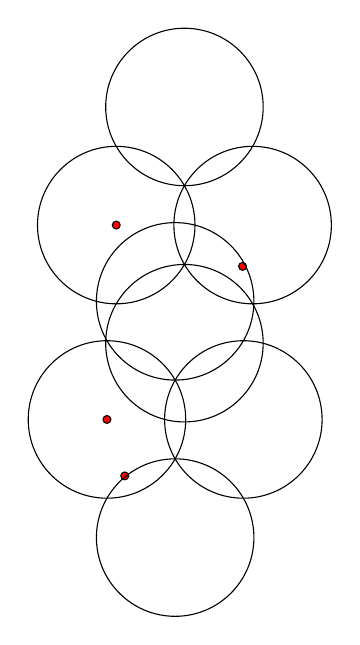
\begin{tikzpicture}

\draw [fill=red,stroke=red] (-0.360984,-0.801107) circle [radius=0.050000];
\draw [fill=red,stroke=red] (-0.243193,1.667566) circle [radius=0.050000];
\draw [fill=red,stroke=red] (-0.135019,-1.517913) circle [radius=0.050000];
\draw [fill=red,stroke=red] (1.360856,1.142937) circle [radius=0.050000];
\draw (-0.360984,-0.801107) circle [radius=1];
\draw (1.371066,-0.801107) circle [radius=1];
\draw (0.505041,0.698893) circle [radius=1];
\draw (0.505041,-2.301107) circle [radius=1];
\draw (-0.243193,1.667566) circle [radius=1];
\draw (1.488858,1.667566) circle [radius=1];
\draw (0.622832,3.167566) circle [radius=1];
\draw (0.622832,0.167566) circle [radius=1];


\end{tikzpicture}

\end{document}